\section{Architecture et Composants}
Pour lire automatiquement les numéros des plaques d’immatriculation, un système ANPR s’étend généralement sur 4 grandes phases:
\begin{enumerate}
    \item \textbf{Acquisition de l’image}: C’est l’entrée de tout système ANPR. A travers une caméra, le système reçoit une séquence d’images.
    \item \textbf{Pré-traitement}: C’est une phase qui est déterminante pour la précision du système. Elle permet d’améliorer la qualité de l’image acquise pour faciliter les prochains traitements.
    \item \textbf{Détection de la plaque}: C’est l’étape la plus importante et en même la plus difficile d’un système ANPR. Elle consiste à identifier sur l’ensemble de l’image la position exacte de la plaque et par la suite l’isoler du reste de l’image. Dans la littérature, plusieurs méthodes ont été proposées pour réussir cette phase à savoir:
        \begin{itemize}
            \item[•] \textbf{La méthode d’extraction des régions d’intérêt}: La région d'intérêt dans une image donnée est la plaque d'immatriculation. Cette région se trouve par
            application d'un concept pour une image donnée, la région contenant une plaque d'immatriculation devra
            nombre maximum de bords par rapport à toute autre partie dans une image. L’application de ce concept à
            tous les segments extraits, les coordonnées de la région requise sont extraites. Ces valeurs de coordonnées
            sont ensuite utilisées pour extraire la plaque d'immatriculation.
            \item[•] \textbf{La méthode basée sur la texture}: La texture est une caractéristique qui peut être utilisée pour détecter les plaques d’immatriculation vue
            que les caractères d’une plaque ont une texture similaires. Dans cet algorithme, on traite les caractères
            d’une plaque comme une texture distincte du reste des objets contenus dans une image. La méthode est
            décomposée en quatre étapes qui sont les suivantes :
                \begin{itemize}
                    \item \textbf{Analyse de la texture de l’image};
                    \item \textbf{Décomposition de l’image en multi-segment};
                    \item \textbf{Choix du masque};
                    \item \textbf{Analyse des composantes connexes}.
                \end{itemize}
            \item[•] \textbf{La méthode basée sur le contour et le gradient}: Les conditions de luminance non uniforme et la distance variable entre la caméra et le véhicule peuvent
            influencer sur le résultat de la détection des plaques d’immatriculation. Pour cela, il existe une méthode
            de détection des plaques d’immatriculation basée sur les caractéristiques du contour et des propriétés des
            caractères. L’algorithme proposé est basé sur les caractéristiques suivantes :
                \begin{itemize}
                    \item Les pixels présentant les caractères de la plaque ont souvent une valeur de contraste plus élevée par rapport aux pixels voisins.
                    \item Le contour des caractères d’une plaque est toujours un contour fermé.
                    \item Il y’ a une relation de voisinage entre les caractères.
                \end{itemize}
            De plus, cette approche qui se base sur le contour et le gradient est composée de cinq processus qui sont :
                \begin{itemize}
                    \item \textbf{Détection de contour};
                    \item \textbf{Sélection des régions candidates de caractères de la plaque d’immatriculation};
                    \item \textbf{Calcul du gradient magnitude des composantes connexes};
                    \item \textbf{Extraction des caractères};
                    \item \textbf{Localisation de la plaque d’immatriculation de véhicules}.\cite{akacemMaster}
                \end{itemize}
            \item[•] \textbf{La méthode basée sur l’apprentissage profond}: Les méthodes précédentes sont dites déterministes car sont implémentées avec des fonctions mathématiques avec des paramètres fixés. A cet effet, dans l'article \cite{doi:10.1177/0361198120954202}, \Citeauthor{doi:10.1177/0361198120954202} proposent une méthode basée sur un modèle de Deep Learning pour la détection des plaques. En effet, à partir une masse de données d’images contenant les plaques d’immatriculation, on réalise un modèle à l’aide des algorithmes de détection des objets (Object Detection). Ce modèle servira par la suite pour détecter les plaques sur de nouvelles images. Cette approche est de plus en plus adoptée car plus efficace par rapport aux approches classiques déterministes.
        \end{itemize}
    \item \textbf{Reconnaissance des caractères}: Encore appelé \acrshort{ocr}, le but de cette phase est d’extraire sous format textuel (alphanumérique), le numéro de la plaque de d’immatriculation.Si certaines méthodes \cite{krimMaster} \cite{10.1155/2018/6737314} utilisent l'approche classique qui passent par 3 phases (prétraitement, segmentation de caractères et reconnaissance de caractères), d’autres \cite{Alahyane2021OpenDF} \cite{doi:10.1177/0361198120954202} par contre optent pour une approche nouvelle en utilisant directement un modèle de réseaux de neurones pour la reconnaissance des caractères sur l'image de la plaque. Toutefois quelque soit la méthode, une étape de post-traitement sur le texte détecté est nécessaire pour faire d'éventuelles corrections sous la base de la norme d’immatriculation des véhicules spécifique au pays. A la fin de la chaîne, le texte obtenu et nettoyé est soit enregistré dans une base de données ou envoyé à un autre système pour un traitement ultérieur.

\end{enumerate}

\begin{figure}[H]
    \centering
    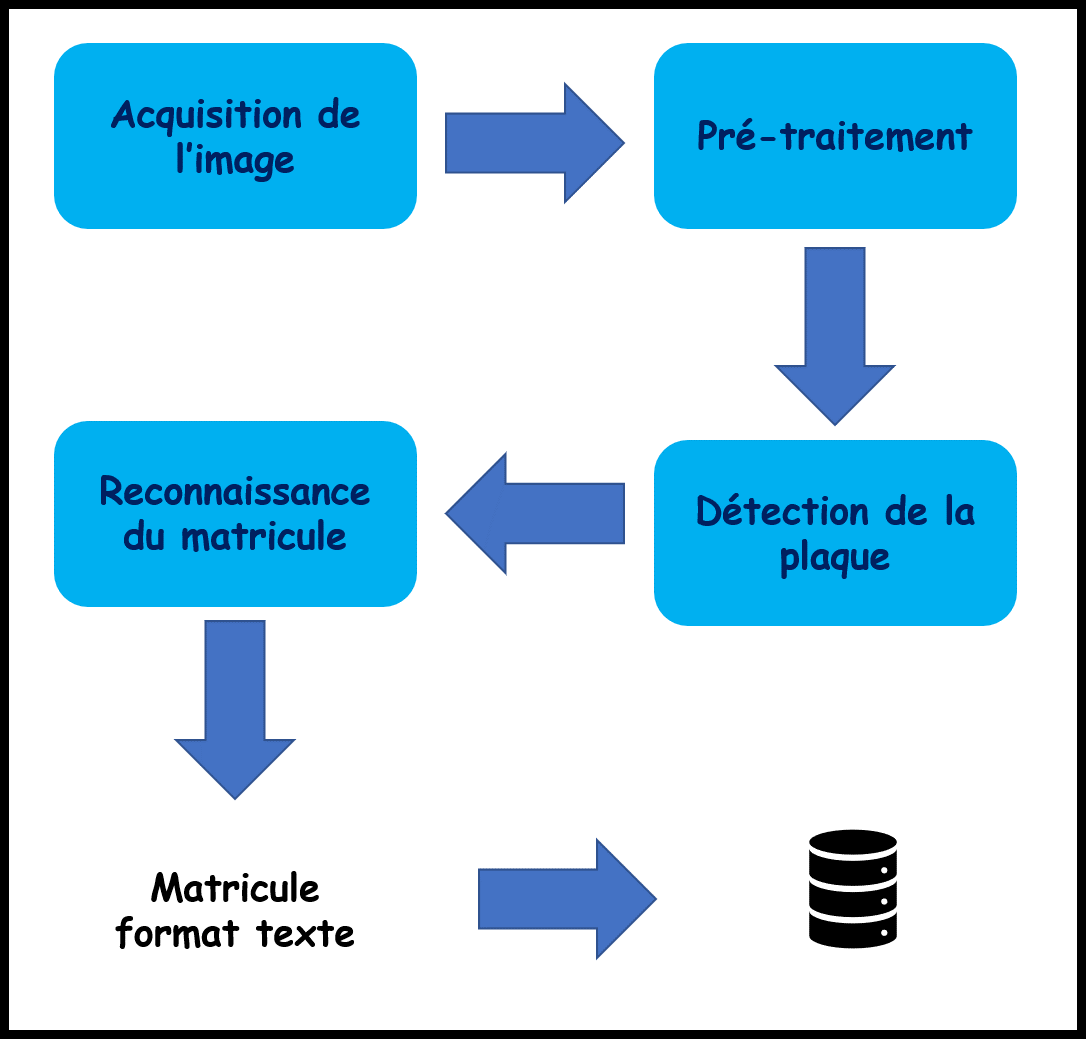
\includegraphics[scale=0.5]{architectureANPR}
    \caption{Architecture de fonctionnement d'un système ANPR}
\end{figure}
Tout système ANPR est constitué essentiellement de deux parties:
    \begin{enumerate}
        \item \textbf{Une partie matérielle}: Elle est composée d’une caméra qui permet d’acquérir les images et d’un ordinateur standard sur lequel s'exécute la partie logicielle du système.
        \item \textbf{Une partie logicielle}: C’est le programme qui traite les images en vue d’extraire les numéros des plaques d’immatriculation. Elle est la plupart du temps liée à une base de données où sont stockées les matricules.
    \end{enumerate}